%%% Hlavní soubor. Zde se definují základní parametry a odkazuje se na ostatní části. %%%

%% Verze pro jednostranný tisk:
% Okraje: levý 40mm, pravý 25mm, horní a dolní 25mm
% (ale pozor, LaTeX si sám přidává 1in)
\documentclass[12pt,a4paper]{report}
\setlength\textwidth{145mm}
\setlength\textheight{247mm}
\setlength\oddsidemargin{15mm}
\setlength\evensidemargin{15mm}
\setlength\topmargin{0mm}
\setlength\headsep{0mm}
\setlength\headheight{0mm}
% \openright zařídí, aby následující text začínal na pravé straně knihy
\let\openright=\clearpage

%% Pokud tiskneme oboustranně:
% \documentclass[12pt,a4paper,twoside,openright]{report}
% \setlength\textwidth{145mm}
% \setlength\textheight{247mm}
% \setlength\oddsidemargin{15mm}
% \setlength\evensidemargin{0mm}
% \setlength\topmargin{0mm}
% \setlength\headsep{0mm}
% \setlength\headheight{0mm}
% \let\openright=\cleardoublepage

%% Použité kódování znaků: obvykle latin2, cp1250 nebo utf8:
\usepackage[utf8]{inputenc}

%% Ostatní balíčky
\usepackage{graphicx}
\usepackage{amsthm}

\usepackage[nottoc]{tocbibind}

%% TODO: Zjistit, jestli je nutné mít v referencích url nebo doi
\usepackage[backend=bibtex8,babel=hyphen,url=false,doi=false]{biblatex}
\addbibresource{my.bib}
\addbibresource{mendeley.bib}

%%
\usepackage{amsmath}
\usepackage{amsfonts}
\usepackage{amssymb}
\usepackage[ruled,vlined,linesnumbered,algochapter]{algorithm2e}
\numberwithin{algocf}{chapter} % lepší číslování algoritmů
\usepackage{todonotes}

%%Moje definované příkazy
\DeclareMathOperator*{\argmax}{arg\,max}
\DeclareMathOperator*{\argmin}{arg\,min}

\mathchardef\mhyphen="2D

%% Balíček hyperref, kterým jdou vyrábět klikací odkazy v PDF,
%% ale hlavně ho používáme k uložení metadat do PDF (včetně obsahu).
%% POZOR, nezapomeňte vyplnit jméno práce a autora.
\usepackage[ps2pdf,unicode]{hyperref}   % Musí být za všemi ostatními balíčky
\hypersetup{pdftitle=Distributed Monte-Carlo Tree Search for Games with Team of Cooperative Agents}
\hypersetup{pdfauthor=Ondřej Filip}

\renewcommand\bibname{References}

%\usepackage{apacite}

%%% Drobné úpravy stylu

% Tato makra přesvědčují mírně ošklivým trikem LaTeX, aby hlavičky kapitol
% sázel příčetněji a nevynechával nad nimi spoustu místa. Směle ignorujte.
\makeatletter
\def\@makechapterhead#1{
  {\parindent \z@ \raggedright \normalfont
   \Huge\bfseries \thechapter. #1
   \par\nobreak
   \vskip 20\p@
}}
\def\@makeschapterhead#1{
  {\parindent \z@ \raggedright \normalfont
   \Huge\bfseries #1
   \par\nobreak
   \vskip 20\p@
}}
\makeatother

% Toto makro definuje kapitolu, která není očíslovaná, ale je uvedena v obsahu.
\def\chapwithtoc#1{
\chapter*{#1}
\addcontentsline{toc}{chapter}{#1}
}


\begin{document}

% Trochu volnější nastavení dělení slov, než je default.
\lefthyphenmin=2
\righthyphenmin=2

%%% Titulní strana práce

\pagestyle{empty}
\begin{center}

\large

Charles University in Prague

\medskip

Faculty of Mathematics and Physics

\vfill

{\bf\Large MASTER THESIS}

\vfill

\centerline{\mbox{\includegraphics[width=60mm]{img/logo.eps}}}

\vfill
\vspace{5mm}

{\LARGE Bc. Ondřej Filip}

\vspace{15mm}

% Název práce přesně podle zadání
{\LARGE\bfseries Distributed Monte-Carlo Tree Search for Games with Team of Cooperative Agents}

\vfill

% Název katedry nebo ústavu, kde byla práce oficiálně zadána
% (dle Organizační struktury MFF UK)
Department of Theoretical Computer Science and Mathematical Logic

\vfill

\begin{tabular}{rl}

Supervisor of the master thesis: & Mgr. Viliam Lisý, MSc. \\
\noalign{\vspace{2mm}}
Study programme: & Theoretical Computer Science \\
\noalign{\vspace{2mm}}
Specialization: & Nonprocedural Programming and \\
                & Artificial Inteligence \\
\end{tabular}

\vfill

% Zde doplňte rok
Prague 2013

\end{center}

\newpage

%%% Následuje vevázaný list -- kopie podepsaného "Zadání diplomové práce".
%%% Toto zadání NENÍ součástí elektronické verze práce, nescanovat.

%%% Na tomto místě mohou být napsána případná poděkování (vedoucímu práce,
%%% konzultantovi, tomu, kdo zapůjčil software, literaturu apod.)

\openright

\noindent
Dedication.

\newpage

%%% Strana s čestným prohlášením k diplomové práci

\vglue 0pt plus 1fill

\noindent
I declare that I carried out this master thesis independently, and only with the cited
sources, literature and other professional sources.

\medskip\noindent
I understand that my work relates to the rights and obligations under the Act No.
121/2000 Coll., the Copyright Act, as amended, in particular the fact that the Charles
University in Prague has the right to conclude a license agreement on the use of this
work as a school work pursuant to Section 60 paragraph 1 of the Copyright Act.

\vspace{10mm}

\hbox{\hbox to 0.5\hsize{%
In ........ date ............
\hss}\hbox to 0.5\hsize{%
signature of the author
\hss}}

\vspace{20mm}
\newpage

%%% Povinná informační strana diplomové práce

\vbox to 0.5\vsize{
\setlength\parindent{0mm}
\setlength\parskip{5mm}

Název práce:
Distribuovaný Monte-Carlo Tree Search pro hry s týmem kooperujících agentů
% přesně dle zadání

Autor:
Bc. Ondřej Filip

Katedra:  % Případně Ústav:
Katedra teoretické informatiky a matematické logiky
% dle Organizační struktury MFF UK

Vedoucí diplomové práce:
Mgr. Viliam Lisý, MSc., Centrum agentních technologií, České Vysoké Učení Technické v Praze
% dle Organizační struktury MFF UK, případně plný název pracoviště mimo MFF UK

Abstrakt: Cílem této práce je návrh, implementace a experimentální evaluace distribuovaných 
algoritmů pro
plánování akcí týmu kooperujících autonomních agentů založených na 
Monte-Carlo tree search algoritmu. Jednotlivé algoritmy vyžadují rozdílné množství komunikace. 
V práci jsou shrnuty relevantní poznatky o Monte-Carlo 
tree search algoritmu, jeho paralelizaci a distribuovatelnosti a
algoritmech pro distribuovanou koordinaci autonomních agentů. Navržené algoritmy jsou testovány
v prostředí zjednodušené hry Ms Pac-Man. Testována je síla jednotlivých algoritmů v závislosti
na času výpočtu, množství komunikace a robustnosti vůči selhání komunikace. Jednotlivé
algoritmy jsou dle těchto charakteristik porovnány.
% abstrakt v rozsahu 80-200 slov; nejedná se však o opis zadání diplomové práce

Klíčová slova:
% 3 až 5 klíčových slov
Multi-agentní systémy, Monte-Carlo Tree Search, distribuované algoritmy


\vss}\nobreak\vbox to 0.49\vsize{
\setlength\parindent{0mm}
\setlength\parskip{5mm}

Title:
Distributed Monte-Carlo Tree Search for Games with Team of Cooperative Agents
% přesný překlad názvu práce v angličtině

Author:
Bc. Ondřej Filip

Department:
Department of Theoretical Computer Scientce and Mathematical Logic
% dle Organizační struktury MFF UK v angličtině

Supervisor:
Mgr. Viliam Lisý, MSc., Agent Technology Center, Czech Technical University in Prague
% dle Organizační struktury MFF UK, případně plný název pracoviště
% mimo MFF UK v angličtině

Abstract: The aim of this work is design, implementaton and experimental evaluation of
distributed algorithms for planning actions of a team of cooperative autonomous agents.
Particular algorithms require different amount of communication. In the work, the related
research on Monte-Carlo tree search algorithm, its parallelization and distributability and
algorithms for disbtributed coordination of autonomous agents. Designed algorithms are tested
in the environment of the game of Ms Pac-Man. Quality of the algorithms is tested in dependence
on computational time, the amount of communication and the robustness against communication
failures. Particular algorithms are compared according to these characteristics.
% abstrakt v rozsahu 80-200 slov v angličtině; nejedná se však o překlad
% zadání diplomové práce

Keywords:
% 3 až 5 klíčových slov v angličtině
Multi-agent systems, Monte-Carlo Tree Search, distributed algorithms

\vss}

\newpage

%%% Strana s automaticky generovaným obsahem diplomové práce. U matematických
%%% prací je přípustné, aby seznam tabulek a zkratek, existují-li, byl umístěn
%%% na začátku práce, místo na jejím konci.

\openright
\pagestyle{plain}
\setcounter{page}{1}
\tableofcontents


%%% Jednotlivé kapitoly práce jsou pro přehlednost uloženy v samostatných souborech
\chapter*{Introduction}
\addcontentsline{toc}{chapter}{Introduction}

\todo{Zatím jen nápady, přepsat, až bude zbytek hotový}



Problem of the coordination of a team of agents is widely discussed topic.
Designing of algorithms for such a coordination meets various difficulties 
including positional information interchanging, distribution of plan computation, 
communication reliability or system failures.

Monte-Carlo Tree Search is a best-first search algorithm which has
reached unprecedent results in playing a game of Go.
Accordingly to the proven qualities of the algorithms further works have
been dealing with it finding applications of the algorithm in various
domains.
Recently a work on team coordination using MCTS has been published by
Nguyen and Thawonmas \cite{Nguyen2011}.
MCTS is applied to controlling a team of ghosts in well-known Pacman
game in this paper.
Their computer player won the CEC 2011 Ms Pac-Man vs Ghost Team
Competition \cite{PacmanVsGhosts}.

\begin{itemize}
\item Nguien's ghosts runs simple instance of algorithm sharing tree
over all agents in team, no communication needed since joint moves are
calculated and passed to the environment
\item Our aim is to develop algorithms based on MCTS giving the autonomy
to agents what brings necessity of communication between agents
\item We consider the domain of Ms Pac-Man vs Ghost Team Competition
suitable for evaluation of the algorithms because the game of Ms Pac-Man
is well-known, frame
\item
\end{itemize}




\chapter{Monte-Carlo Tree Search}
\label{chap_mcts}

Mone-Carlo Tree Search (MCTS) is an iterative best-first search algorithm with stochastic positional
evaluation, anytime property and fast convergence. As \citeauthor{ChaslotPhd2010} summed up in 
\cite{ChaslotPhd2010}, MCTS was simultaneously developed
in three variants (\cites{Chaslot2006}{Coulom2006}{Kocsis2006}) in 2006. Specific variant used in
this thesis along with all important details and explanation of the properties is discussed in this
chapter.


\section{Algorithm Description}

\citeauthor{Chaslot2008} provides good description of the Monte-Carlo Tree Search algorithm in
\cite{Chaslot2008}. Variant of MCTS as well as the terminology used in this thesis are based mainly
on this paper.

Monte-Carlo Tree Search is iteratively building the search tree as depicted by picture
\emph{TODO}%\ref{fig_mcts_phases}
 and algorithm \ref{alg_mcts_loop}. Nodes of the tree contains at least two values - visit count
 saying how many random evaluations of positions in node's subtree have been executed and actual
 value which aggregates actual values from node's subtree (usually the average).

Each iteration of MCTS consists of four
phases - \emph{selection}, \emph{expansion}, \emph{simulation} and \emph{backpropagation}. During
the selection phase the 
algorithm passes through the tree to a particular leaf where better-evaluated but less-visited nodes
are preferred. Appropriate balance between these contradictory claims is main objective of this
phase. Once a leaf node is selected the expansion phase follows and all children nodes reachable
from the leaf node with one valid move are added to the leaf and one of these children is chosen.
The next phase, simulation (also called playout), plays a random game (or several ones) starting
in position defined by expanded node halting on some conditions (e.g. after certain moves are
played, the end of the game is reached). Results from the simulations are then backpropagated to all
expanded node's ancestors during the fourth phase (backpropagation). The phases of the algorithm are
further discussed in subsequent sections.

\begin{algorithm}
\DontPrintSemicolon
\caption{Monte-Carlo Tree Search\label{sec_mcts_description}}
\label{alg_mcts_loop}
$tree \leftarrow new\,McTree()$ \tcp*[h]{Initialize empty tree}\;
$root \leftarrow Root(tree)$\;
\While(\tcp*[h]{Main MCTS loop}){$EnoughTime()$}{
    $last\_node \leftarrow root$ \tcp*[h]{Phase 1: Selection}\;
    \While{$curr\_node \in tree$}{
        $last\_node \leftarrow curr\_node$\;
        $curr\_node \leftarrow Select(curr\_node)$\;
    }
    $last\_node \leftarrow Expand(last\_node)$ \tcp*[h]{Phase 2: Expansion}\;
    $reward \leftarrow Playout(last\_node)$ \tcp*[h]{Phase 3: Simulation}\;
    \While(\tcp*[h]{Phase 4: Backpropagation}){$curr\_node \in tree$}{
        $reward \leftarrow Backpropagate(curr\_node,\:reward)$\;
        $N_{curr\_node} \leftarrow N_{curr\_node}+1$ \tcp*[h]{Increase node's visit count}\;
        $curr\_node \leftarrow Parent(curr\_node)$\;
    }
}
\Return{$\argmax\limits_{n \in Children(root)}(N_{n})$} \tcp*[h]{Return most visited child}\;
\end{algorithm}


\subsection{Selection}

The process of selection consists of selection steps passing from a node to one of it's children.
Each such a step meets exploration-exploitation contradiction where exploitation tends to choose the
best node (one with the greatest current value) and exploration on the other side promotes
undiscovered ways in the tree. This problem is well-known as the Multi-Armed Bandit Problem (MAB)
\cites{Auer2002}{Kocsis2006}. 

\emph{XXX: Vadí (téměř) doslovný přepis definice?}

\begin{samepage}
\newtheorem*{defmab}{Definition}
\begin{defmab}[K-armed bandit problem ] 

Let us have independent random variables $X_{i,n}$ for $1 \le i \le K$ and $n \ge 1$. Each $i$ is
the index of a gambling machine and $X_{i,1}$, $X_{i,2}$,\ldots are identically distributed rewards
with unknown expected value $\mu_i$ yielded by successive plays of machine $i$. For the simplicity
the rewards are bounded to $[0,1]$.

A policy $A$ is an algorithm that chooses the next machine to play based on the sequence of
past plays and obtained rewards. Let $T_i(n)$ be the number of times machine $i$ has been played by
$A$ during the first $n$ plays and $I_i^A$ be the index of a machine played in nth play. Then the
regret of A after n plays is defined as

\begin{equation}
R_n^A = n \mu^* - \sum_{j=1}^K T_j(n) \mu_j \mathrm{,\;where}\;\mu^* \stackrel{\mathrm{def}}{=}
\max_{1 \le i \le K} \mu_i
\end{equation}

thus the regret $R_n^A$ is the loss caused by the policy not always playing the best machine.

K-armed bandit problem consists in finding optimal policy $A^*$ minimizing
expected regret $R_n^A$.

\end{defmab}
\end{samepage}

\emph{TODO: co citovat? Originální knížku z roku 85 nebo \cite{Auer2002}, kde se na ní odkazují?}
\emph{TODO: až se vyřeší citace, doplnit zmínku o tom, že optimální policy má regret  ~$O(log(n))$,
ale že je výpočetně náročná}

\Citeauthor{Auer2002} introduced computationaly effective optimal policy UCB1 (\cite{Auer2002}) having
regret bounded to $O(log(n))$ defined as:

\begin{equation}
 I_{UCB1}(n+1) = \argmax\limits_{i\in{1,\ldots,K}} \left({\bar{X}_{i,T_i(n)} 
+ \sqrt{{2 \log (n)} \over T_i(n)}}\right)
 \end{equation}.

Abbreviation UCB stands for \emph{Upper-Confidence Bound} and refers to value maximized by the
policy. UCB consists of average of previous rewards and a bias growing decreasing with number of the
machine's plays. In addition significance of the bias is growing with the total number of plays what
leads to increase of exploration.

UCB applied to Trees \cite{Kocsis2006} is derived from UCB using values $v_i$ and $n_i$ stored in
particular node $i$. In addition bias coefficient C is introduced in \cite{Chaslot2008} so the form of
UCT1 describing selection on node $p$ is:

\begin{equation}
I_{UCT1}^p = \argmax\limits_{i \in Children(j)} \left( v_i + C \sqrt{\log{n_p} \over{n_i}}\right)
\end{equation}

where 

 adopting a piece of
generalization in form 

\subsection{Expansion}


\subsection{Simulation}


\subsection{Backpropagation}



\section{Convergence to Minimax algorithm}
\label{sec_minimax_convergence}

\section{MCTS for Two-Player Games}
\emph{Discussion about simultaneous v. turn-based games and its convergence}

\section{Parallel Monte-Carlo Tree Search}








\chapter{Distributed Team Cooperation}
\emph{Extraction from the related chapters from \ref{MAS2008}}
\section{Distributed Constraints Optimization}

\section{Inter-Agent Communication}
\section{Conclusion}

\chapter{Evaluation of Distributed MCTS Algorithms}

\section{Ms.Pacman vs Ghosts Framework}

\section{Design Notes}

\section{Methodics}

\section{Results}

\chapter{Evaluation of Distributed MCTS Algorithms}

\todo{Úvod ke kapitole, co tu bude atd..}

\section{Ms Pac-Man vs Ghosts Framework}

For the purposes of evaluation of algorithms proposed in Chapter \ref{chap_dmcts_design}, we
have chosen the Ms Pac-Man vs Ghosts Framework (\ref{PacmanVsGhosts}) which is easy-to-use
framework allowing implementation of players for well-known old game Pac-Man in Java. Here we
will extract basics of the game rules used in the framework and afterwards we will
describe modifications of the rules we have done and reasons for them.

\subsection{Game rules}

Ms Pac-Man is a game played in a maze in which two sides compete, the Pac-Man and four ghosts.
There are pills everywhere in the maze and Pac-Mans purpuse is to gather all the pills, each
for 10 points. Once all the pills are eaten, the game continues in a next maze. To complicate
the life of Pac-Man, ghosts are moving around the maze pursuing the Pac-Man and trying to
minimize its score. If the Pac-Man is caught, it will lose one life and if has any life
remaining, starts again from its starting position. Pills remain eaten after the life loss.
Ghosts appear in so-called lair at the beginning of each round and after Pac-Man's life loss
from where they start after a several time (different for each ghost). Beside regular pills,
each maze contains four power pills which are awarded with 50 points and when eaten by Pac-Man,
ghosts become edible and twice slower for certain period of time. Pac-Man can eat ghosts during 
this period for
reward of 200 points for first eaten ghost and 400, 800 and 1600 points for other ghosts.
Eaten ghost starts in lair again.

Exact rules of the Ms Pac-Man vs Ghosts game can be found on the project webpage. The game was
additionally modified for purposes of testing of our algorithms. Biggest change of rules is
removing power pills from the mazes together with entire edible ghosts mechanism. Reason for
this decision is lowering the variability of results. When Pac-Man is pursuing edible ghosts,
there is big difference in score when it eats different number of ghosts. For the same reason
three more modification have been done. Pac-Man has only one life, game ends after the first
maze is cleared and random ghosts' reversal is suppressed what is a rule
which adds stochasticity to the game. If the rule is on, there is a 0.15\% probability each tick of
a game that all
ghosts accidentally change their direction. \todo{max. délka hry}
An example of a situation from the game without
power pills is depicted by Figure \ref{fig_pacman_framework}.

\begin{figure}
\begin{center}
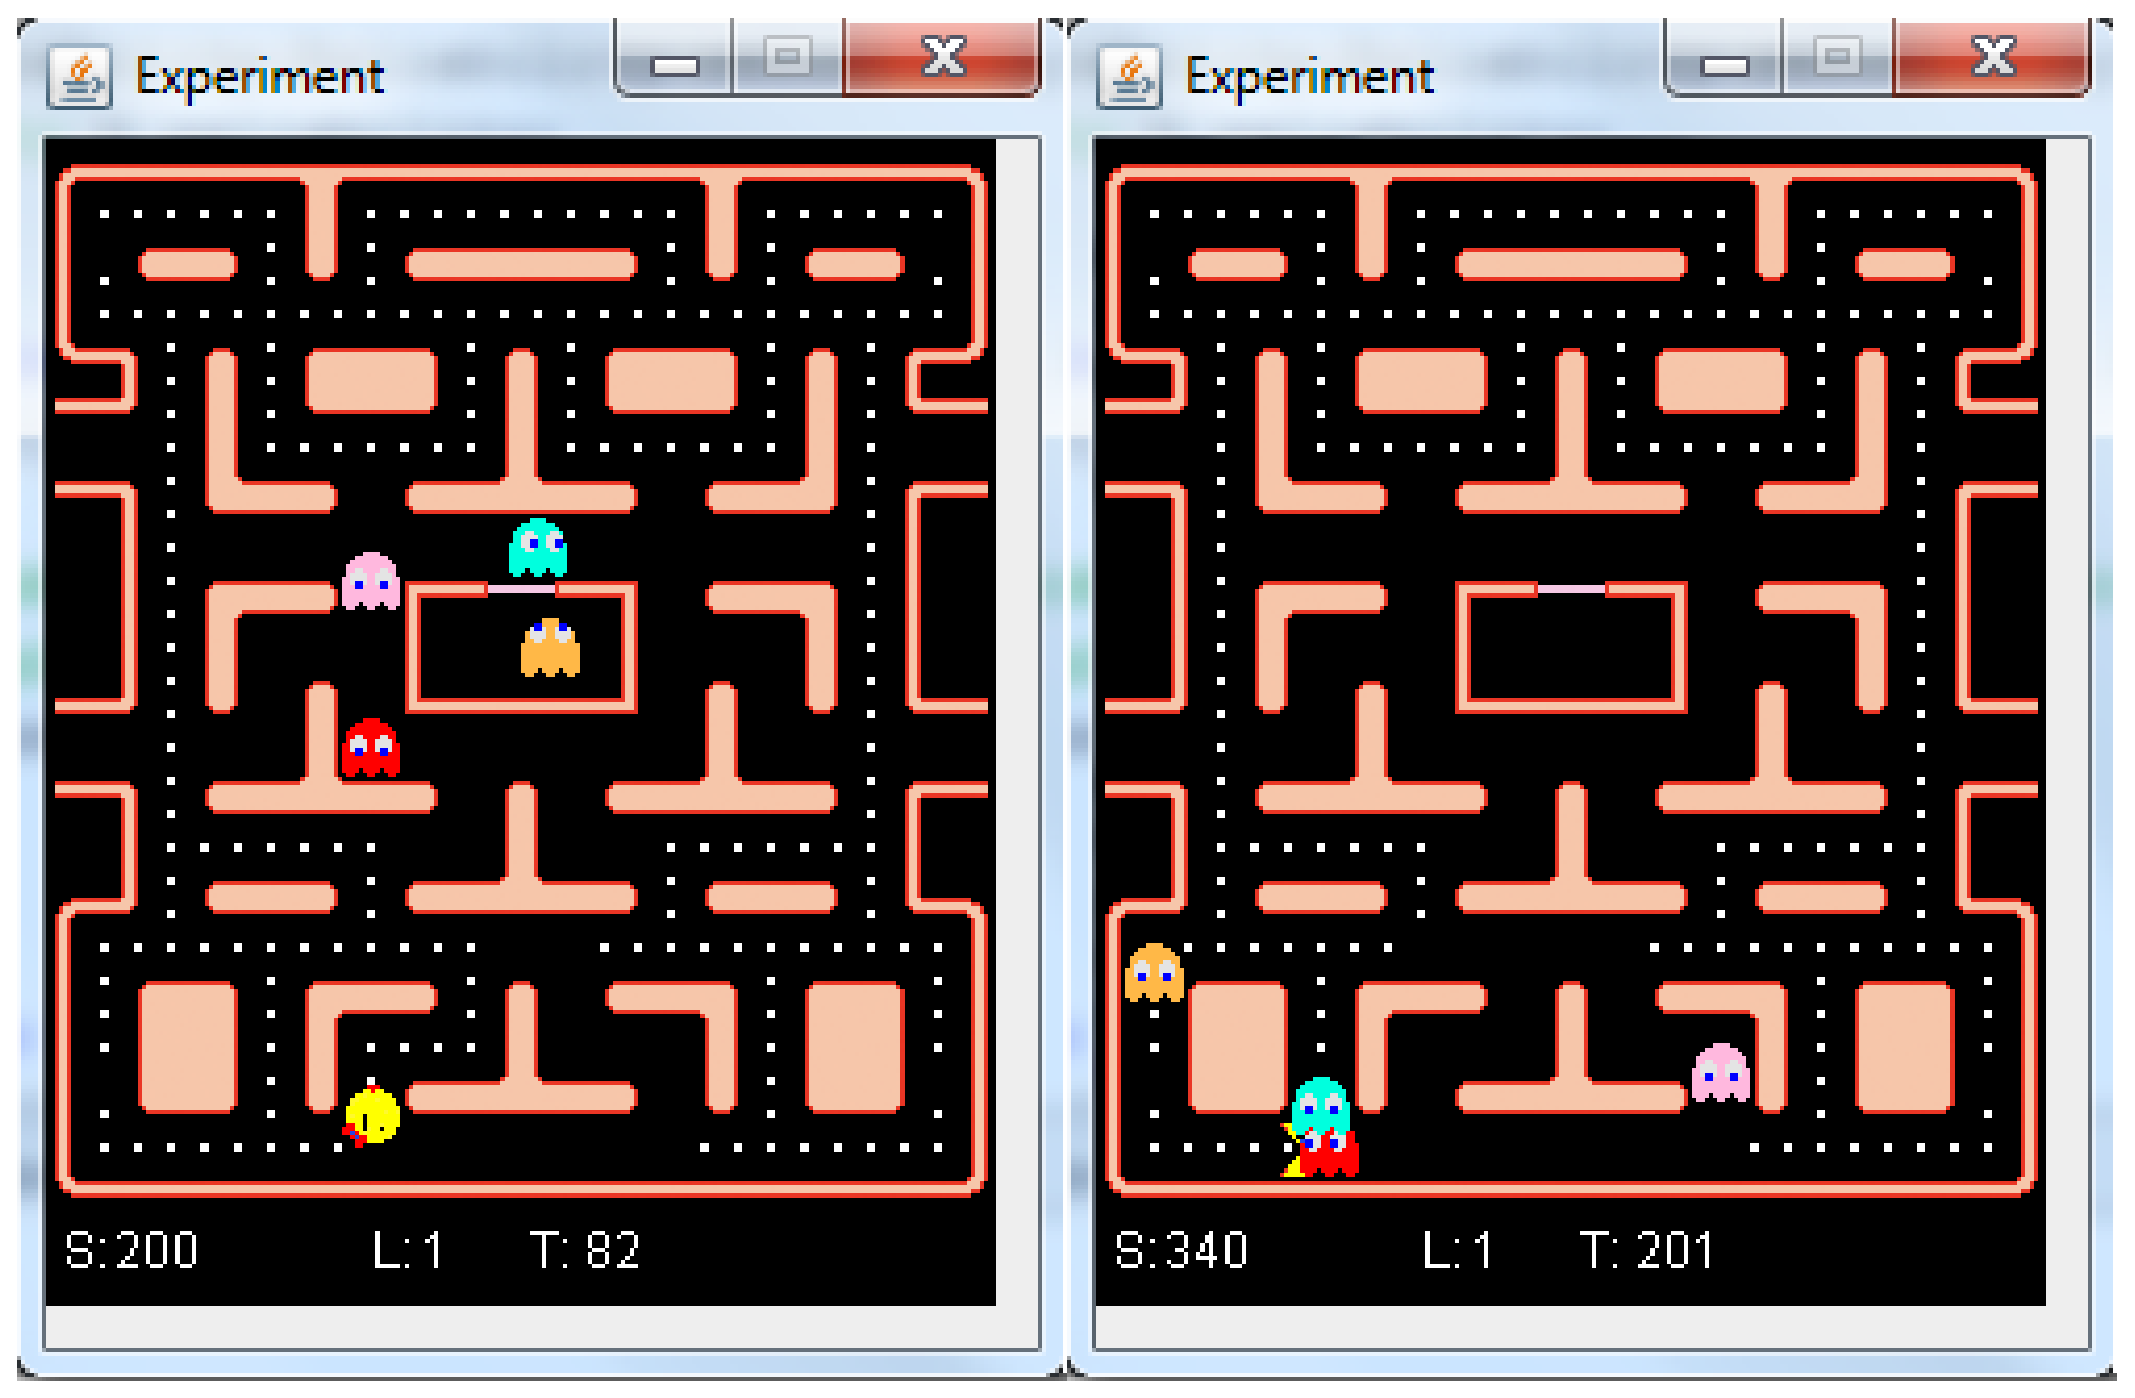
\includegraphics[width=14cm]{img/pacman_framework.eps}
\end{center}
\caption{\footnotesize Game of Ms Pacman.}{\footnotesize Left picture shows the game few moments after it began. Three
ghosts started to hunt the Pac-Man while the orange one is still waiting in lair. Right
picture, on the other hand, shows the game just before the end. Pac-Man does not have any
escape path and is being caught with in a while with no life remaining.}
\label{fig_pacman_framework}
\end{figure}

Pac-Man has the same movement speed as non-edible ghosts. Paths inside the maze are divided
into small segments, four between two neighbouring pills. Pac-Man has to play an action after
at each segment, turning back in the middle of path or at the crossroad is allowed and so
Pac-Man has always at least two action to choose between. Contrarily, ghosts' movement is
restricted. Additional rule on ghosts' movement is that ghosts cannot turn back in the middle
of a path nor at a crossroad. That means that once a ghost chooses one way from a crossroad, it
has to continue to the end of the path. Despite of that, ghosts have to play an action on each
segment even though there is only one action to choose from.

\todo{Porovnat Pac-Mana s pursuit-evation game}

So Pac-Man and ghosts play their actions at each segment of the maze but they, of course, have
to play an action in a limited time. Ms Pac-Man vs Ghosts framework provides by default 40 ms
to play what corresponds with the natural game timing when a human player controls Pac-Man.

\subsection{Framework details}

In our thesis, we use Ms Ghost vs Pacman framework version 6.2. The framework is written in
Java what simplifies the development of controllers of the players. In original game, player
was able to control only Pac-Man and ghosts were controlled by simple AI. In the framework,
it is also possible to develop controller for the ghosts. The only work a user is supposed to 
do is
implement a controller of Pac-Man or ghosts, methods for running a game or a set of games are
prepared for usage. 

A player controller is a class implementing an interface having only one
method. In case of ghosts controller, method's header is \texttt{public EnumMap<GHOST,MOVE>
getMove(Game game,long timeDue)}, where \texttt{EnumMap<GHOST,MOVE>} is a joint-action of
ghosts, \texttt{game} contains information of current game and \texttt{timeDue} contains time
until which the method has to return an action.
If an action is not returned on time, certain
default action is chosen by framework itself.

\todo{Tady je možné ještě popsat, že jsem si upravil i metody na běh experimentů}

\subsection{Pac-Man Opponent}

To evaluate the strength of ghost controllers based on distributed MCTS algorithms, we need to
choose appropriate Pac-Man opponent to play against. Unfortunately, experiments with Pac-Man
controllers included in Ms Pacman vs Ghosts framework showed that these controllers are too
weak for evaluation. Thus, it was necessary to look for better Pac-Man controllers. 

Main purpose of the Ms Pacman vs Ghosts project is organizing competitions between existing
controllers. Competitions are usually held on various conferences and meanwhile there is also a
league  in which all controllers commited into the website compete. Thanks to the leagure
results we were able to contact authors of the league leading Pac-Man and obtained source code
of ICEP\_IDDFS \ref{IcepIddfs} what is controller based on iterative deepening depth-first
search approach. We haven't received more details about the controller. However, experiments
running against it give promising results and so the controller was chosen as an opponent to
compare with.


\section{Implementation Notes}

In this section, we will discuss important implementation details of our controllers. As
mentioned in previous section, framework used for the experiments is written in Java and so
controllers are also supposed to be written in this language.


\subsection{Tree construction}

Here we will talk about the way the concrete realization of MCTS tree for the game of Ms
Pac-Man. The most direct approach to a construction is to keep a node of the tree for each game
step and store, besides the value and the visit count, actions performed by Pac-Man and all
ghosts. By exposing and resolving of problems of this solution, we have reached the
construction used in our controllers.

First problem to be solved is that MCTS tree should not work with simultaneous plays of
multiple teams as discussed in \ref{sec_two_players_mcts}. Section 
\ref{sec_turn_based_game_conversion} gives us a recipe to deal with simultaneous moves by
convertion of a simultaneous game to a turn-based game by splitting simultaneous nodes. The
conversion is not done on the unterlying Ms Pac-Man game itself but only for purposes of
expansion of nodes. When a simultaneous node is being expanded, instead of creating of a child
node for each pacman-ghosts joint-action, only children for each pacman action is created and
each of this children is immediately expanded with ghosts actions. By this approach,
simultaneous nodes are splitted accordingly to optimistic expansion since in such a tree the
ghosts suppose to know the action of Pac-Man played in the simultaneous node. Our
implementation, in addition, supports the pesimistic expansion where ghosts actions are
expanded first in simultaneous nodes.

Second problem is quite high branching factor caused by Pac-Man which is able to change its
direction any time. To reduce the branching factor, we consider additional rules of Pac-Man's
movement for purposes of node expansion. We allow Pac-Man to change its direction only at
crossroads, in the neighbourhood of a segment with not yet eaten power pill and at segments in
the middle of path when last segment allowing the direction change is exactly 6 segments far.
When computing the MCTS tree for Pac-Man, this reduction does not bring any difficulty since
the player controlled by the algorithm follows additional rules. But when Pac-Man is an
opponent of the algorithm, it may play an action not corresponding with these rules what
directly leads to desynchronization between game state and built tree. Next time any ghost
reaches  a crossroad and the desynchronization is detected, ghost play an action accordingly to
the tree but then instead of using a subtree defined by the action for further computations,
new tree is built from scratch.

Finally, after expansion of simultaneous nodes and reduction of Pac-Man moves, the tree
will contain nodes having only one child which are also removed what adds a necessity to keep
lengths of edges between nodes.


\subsection{Pac-Man Playout}

In our work, we decided to keep the simulation strategy simple, not leveraging much of
domain-specific information. This decision is driven by experiments from early phases of
development. During this experiments, both Pac-Man and ghosts players were, with a certain
probability, led by some heuristic algorithm inspired by original legacy behaviour in case of
ghost player and the StarterPacman example controller which is provided as a part of framework.
With supplementary probability, players performed random actions. Because we haven't discovered
any significant strength gain by tuning of the probability of heuristic steps, we omitted
heuristics at all.

The only additional knowledge put into the simulation strategy is that Pac-Man is not allowed
to change its direction in the middle of a path during simulation. The point of this 
restriction is that once Pac-Man enters a path, it usually wants to continue to a next
crossroad. In addition, such a restriction heightens expected size of area visited by Pac-Man
because situations of Pac-Man idling in the middle of path are suppressed.


\subsection{Communication}

Main method of a player controller (\texttt{getMove}) returns the joint-action
(\texttt{EnumMap<GHOST,MOVE>}) of the ghosts
but for purposes of distributed approach, each ghost is supposed to reason individually 
returning its action. To fulfil this, four subcontrollers, returning single \texttt{MOVE}
actions are started in four separated threads and virtual bidirectional communication 
channels are created between each pair of subcontrollers.

Channels provide interfaces for both senders and receivers and work with real time. Channel
consists of queue of messages to be sent and queue of received messages. Messages from the
sending queue to the receiving queue are transmitted every time a method on a channel is
called. Amount of messages transmitted corresponds with time elapsed since last channel event
ending with nonempty sending queue.

For purposes of evaluation of robustness of distributed algorithms againts communication
failures, channels contain a reliability object which simulates a reliability of a channel.
After a transmission of each message, the object determine if the message is really transmitted
to the receiver or if a failure occured and the message has to be discarded. Exact way of
reasoning of the reliability object is described in Section \ref{sec_methodics}.



\section{Methodics}
\label{sec_methodics}

All experiments were performed in virtualized environment of CentOS release 6.3 (Final) having
assigned 12 CPUs and 16 GiB of memory. Underlying host server disposes of 2 Intel(R) Xeon(R) 
CPU E5-2630 0 @ 2.30GHz processors (6 cores/12 threads each) and total of 128 GiB of memory.
Beside of our testing server, a few other virtual servers were running on the host server with
a light consumption of resources but taking into account that we were leveraging at most 4
cores at a time, remaining cores could easily handle the traffic. 

\todo{Turbo boost??}

Java runtime used for experiments is \texttt{1.7.0\_09-icedtea}.

Simple bash scripts were used for purpuses of launching of individual games. Our Java
application contains uniform entry point allowing setting of necessary parameters for running
of an experiment. Each experiment were performed 100 times and average values were then used.
Data gathered during experiments were then processed in R environment. Graphs contained in this
work are also generated with R.

\section{MCTS Tuning}

\begin{figure}
\begin{center}
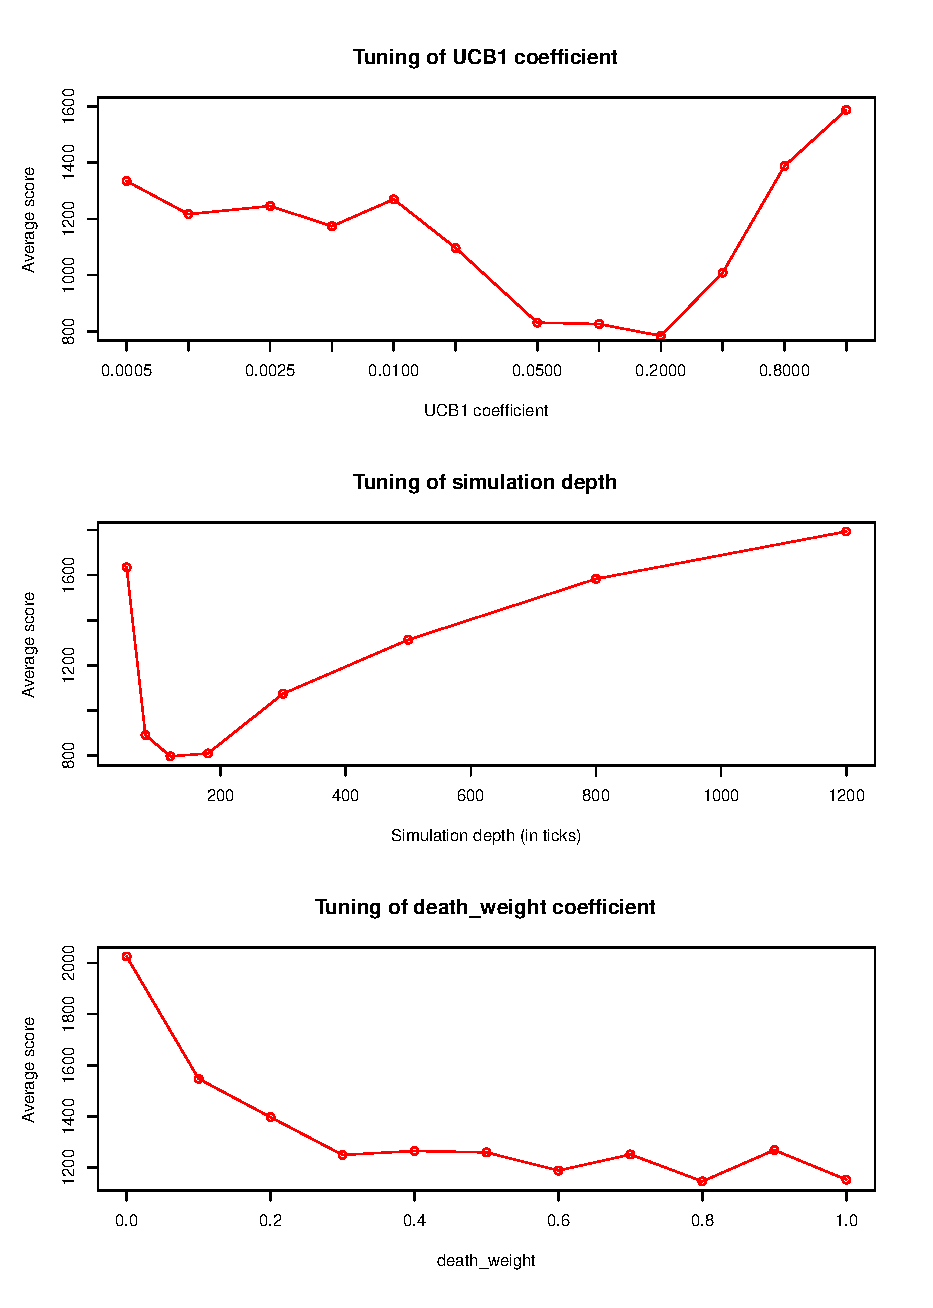
\includegraphics{img/mcts-tuning.eps}
\end{center}
\caption{\footnotesize Lorem ipsum}{\footnotesize }
\label{fig_mcts_tuning}
\end{figure}


\section{Comparison of the Algorithms}

\subsection{Centralized Monte-Carlo Tree Search}

\begin{figure}
\begin{center}
\includegraphics{img/plain-mcts-strength.eps}
\end{center}
\caption{\footnotesize Lorem ipsum}{\footnotesize }
\label{fig_plain_mcts_strength}
\end{figure}

\subsection{Independent Agents}

\begin{figure}
\begin{center}
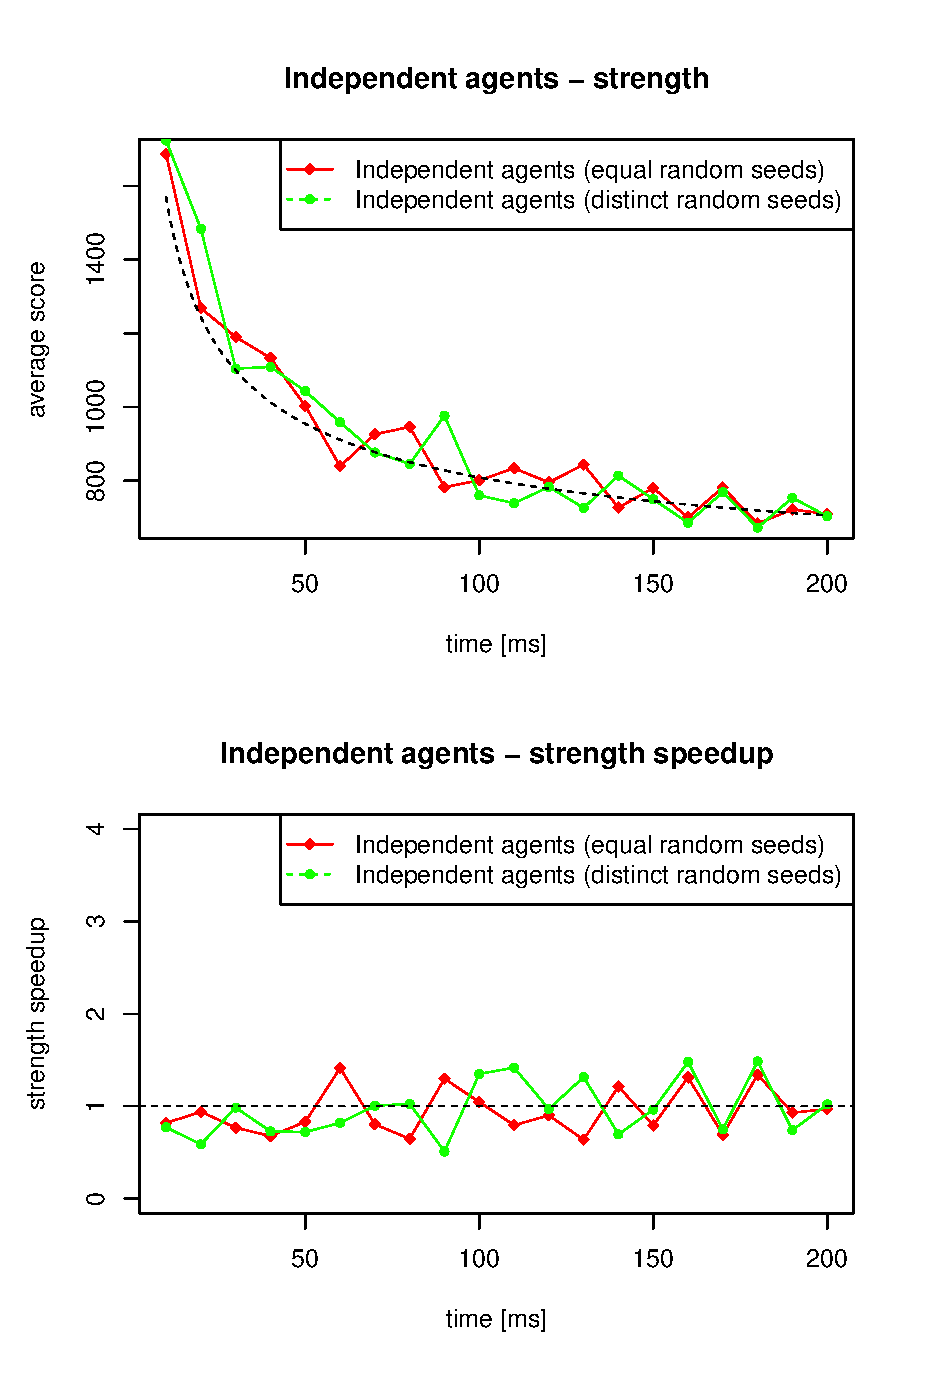
\includegraphics{img/dummy-ghosts-strength.eps}
\end{center}
\caption{\footnotesize Lorem ipsum}{\footnotesize }
\label{fig_independen_agents_strength}
\end{figure}

\subsection{Join-Action Exchanging Agents}

\begin{figure}
\begin{center}
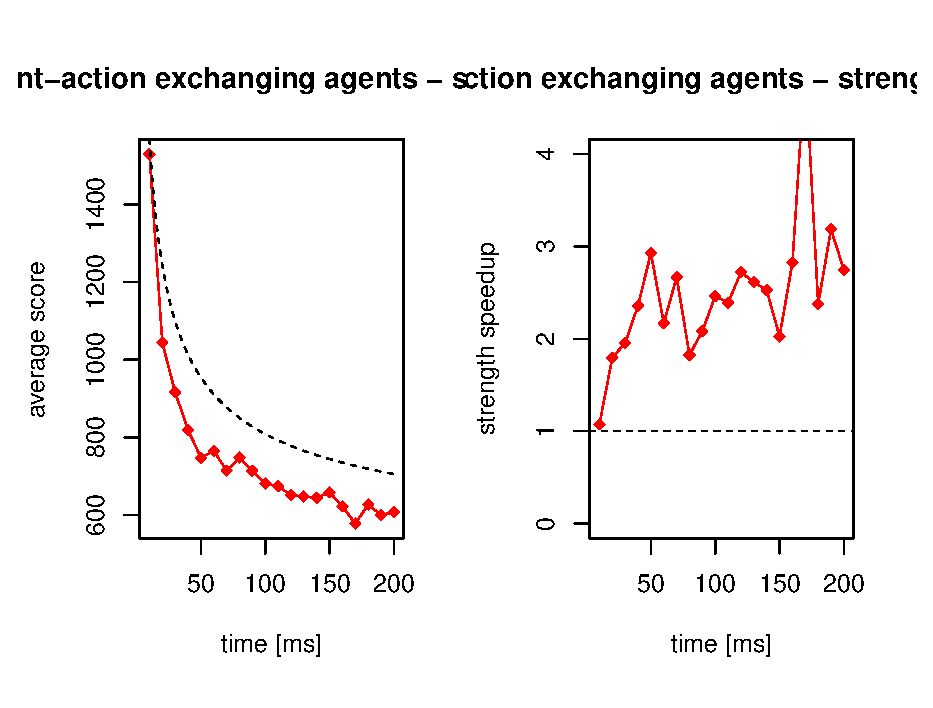
\includegraphics{img/move-exchange-strength.eps}
\end{center}
\caption{\footnotesize Lorem ipsum}{\footnotesize }
\label{fig_action_exchanging_strength}
\end{figure}

\subsection{Root Exchanging Agents}

\begin{figure}
\begin{center}
\includegraphics{img/root-exchange-strength.eps}
\end{center}
\caption{\footnotesize Lorem ipsum}{\footnotesize }
\label{fig_root_exchanging_strength}
\end{figure}

\subsection{Simulation Results Passing Agents}

\begin{figure}
\begin{center}
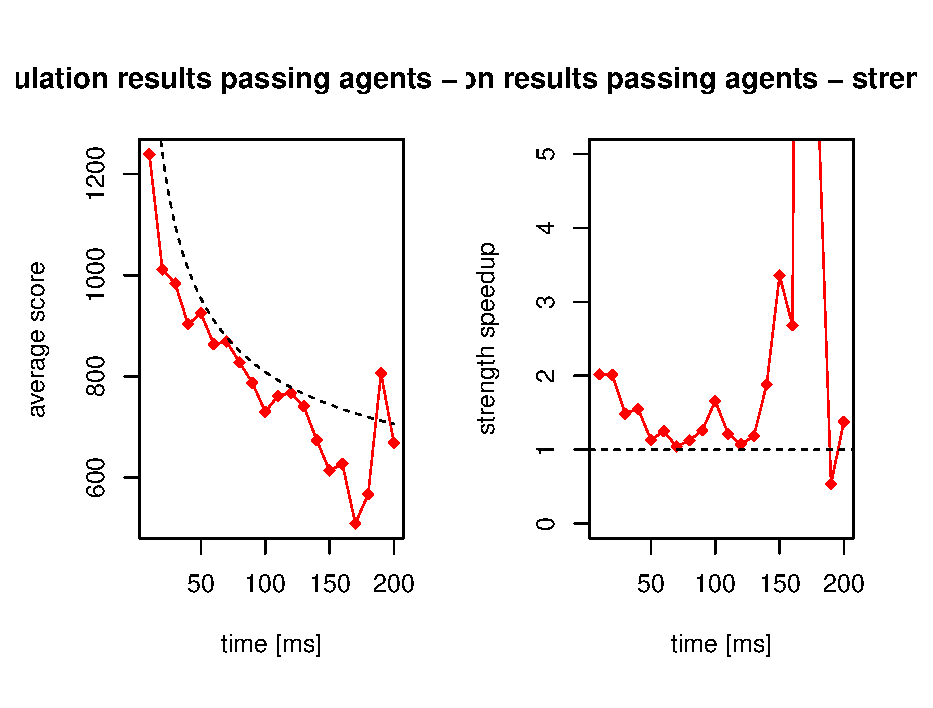
\includegraphics{img/simulation-passing-strength.eps}
\end{center}
\caption{\footnotesize Lorem ipsum}{\footnotesize }
\label{fig_simulation_passing_strength}
\end{figure}

\begin{figure}
\begin{center}
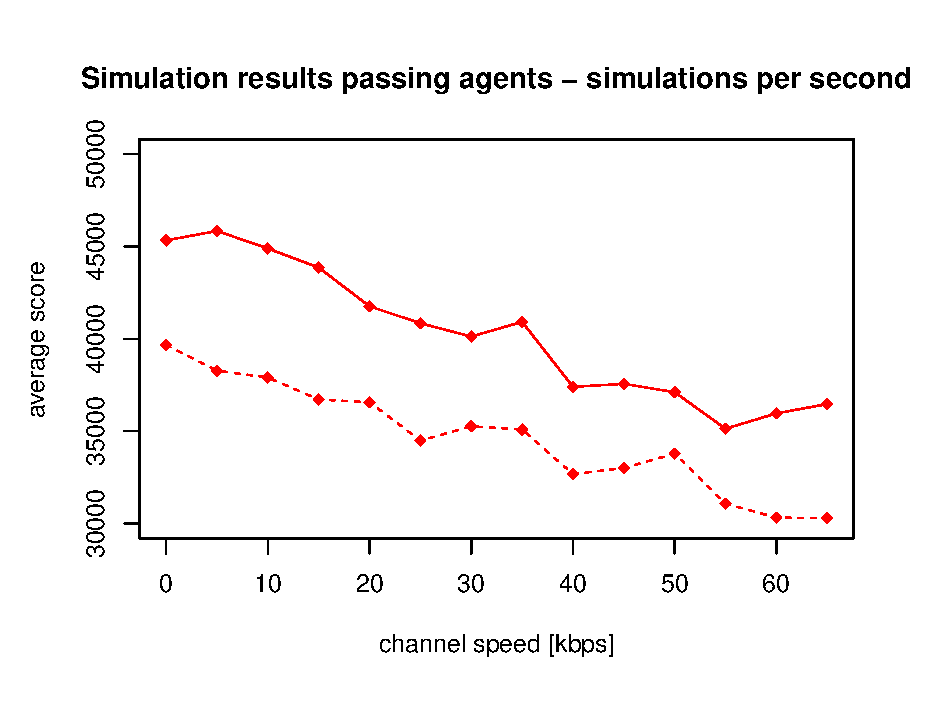
\includegraphics{img/simulation-passing-sims-per-sec.eps}
\end{center}
\caption{\footnotesize Lorem ipsum}{\footnotesize }
\label{fig_simulation_passing_sims_per_sec}
\end{figure}

\subsection{Tree-Cut Exchanging Agents}

\begin{figure}
\begin{center}
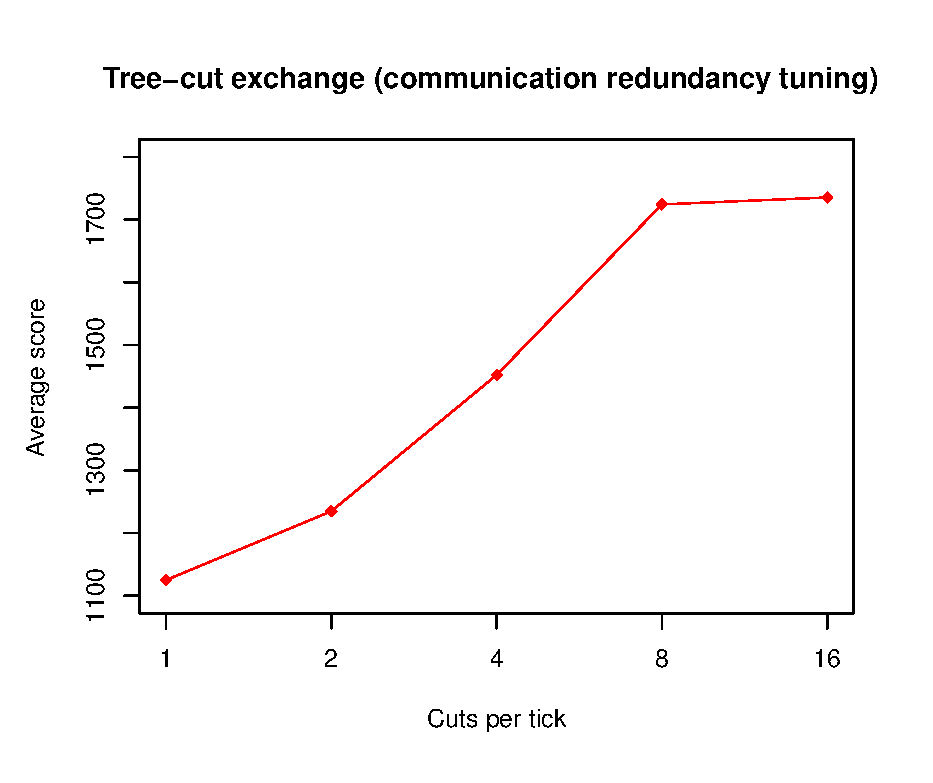
\includegraphics{img/tree-cut-tuning.eps}
\end{center}
\caption{\footnotesize Lorem ipsum}{\footnotesize }
\label{fig_tree_cut_tuning}
\end{figure}

\subsection{Comparison}

\section{Conclusion}


% Ukázka použití některých konstrukcí LateXu (odkomentujte, chcete-li)
% \include{example}

\chapter*{Conclusion}
\section*{Summary}
\section*{Future Work}
\addcontentsline{toc}{chapter}{Conclusion}


%%% Seznam použité literatury
%%% Seznam použité literatury je zpracován podle platných standardů. Povinnou citační
%%% normou pro diplomovou práci je ISO 690. Jména časopisů lze uvádět zkráceně, ale jen
%%% v kodifikované podobě. Všechny použité zdroje a prameny musí být řádně citovány.
%
%def\bibname{Bibliography}
%begin{thebibliography}{99}
%addcontentsline{toc}{chapter}{\bibname}

%\bibitem{mas2008} 
%{\sc Shoham} Yoav, {\sc Leyton-Brown} Kevin.
%\emph{Multiagent Systems: Algorithmic, Game-Theoretic, and Logical Foundations}
%Revision 1.1
%Cambridge University Press, 2008.

%end{thebibliography}
%\bibliography{bibliography}
%\bibliography{plain}
%\nocite{Chaslot2008}
%\nocite{Nguyen2011}
\nocite{Chaslot2008}
\nocite{MAS2008}
\nocite{Nguyen2011}
\nocite{Bouzy2007}

%\bibliographystyle{apacite}
%\bibliographystyle{plain}
%\bibliography{mendeley,my}
\printbibliography


%\include{bibl}

\listoftodos

%\chapwithtoc{List of Algorithms}

%%% Tabulky v diplomové práci, existují-li.
%\addcontentsline{toc}{chapter}{List of Tables}
\listoftables

%\addcontentsline{toc}{chapter}{List of Figures}
\listoffigures

\listofalgorithms
\addcontentsline{toc}{chapter}{List of Algorithms}

%%% Použité zkratky v diplomové práci, existují-li, včetně jejich vysvětlení.
\chapwithtoc{List of Abbreviations}

\begin{tabular}{ll}
MCTS & Monte-Carlo tree search \\
UCB & Upper-confidence bound \\
UCT & UCB for trees \\
\end{tabular}

%%% Přílohy k diplomové práci, existují-li (různé dodatky jako výpisy programů,
%%% diagramy apod.). Každá příloha musí být alespoň jednou odkazována z vlastního
%%% textu práce. Přílohy se číslují.


\chapwithtoc{Attachment 1 -- DVD Contents}
\label{att_dvd_contents}i
\todo{Refer here from Preface or summary}
\todo{!}

\chapwithtoc{Attachment 2 -- Software Work}
\label{att_software}
\todo{Attachment - software documentation, cite it in Implementatin Details section}

\openright
\end{document}
